\documentclass{beamer}
\usepackage{graphicx}
\graphicspath{img}

\title{Causal Diagrams and the Identification of Causal Effects}
\author{Mingyu Liu}
\date{Oct 26th, 2022}

\begin{document}
\frame{\titlepage}

\begin{frame}
\frametitle{Preface}
\begin{itemize}
\item \textbf{Previous Chapter:} dealt with ways of learning causal relationships from raw data
\item \textbf{This Chapter:} explore the ways of inferring such relationships from a combination of data and qualitative causal assumptions that are deemed plausible in a given domain
\item Uses \textbf{causal diagrams} to give formal semantics to the notion of intervention, and it provides explicit formulas for postintervention probabilities in terms of preintervention probabilities
\item The implication is that the effects of every intervention can be estimated from nonexperimental data (provided the data is supplemented with a causal diagram that is acyclic and contains no latent variables)
\end{itemize}
\end{frame}

\begin{frame}
\begin{itemize}
\item If some variables are not measured then the question of \textbf{identifiability} arises, and this chapter develops a nonparametric framework for analyzing the identification of causal relationships in general and causal effects in particular
\item Causal diagrams provide a powerful mathematical tool -- they can be \textbf{queried}, to determine if the assumptions available are sufficient for identifying causal effects
\begin{itemize}
  \item If so, the diagrams produce \textit{mathematical expressions for causal effects} in terms of observed distributions
  \item Otherwise, the diagrams can be queried to suggest \textit{additional observations or auxiliary experiments} from which the desired inferences can be obtained
\end{itemize}
\end{itemize}
\end{frame}

\begin{frame}
\begin{itemize}
\item Example: Smoking and the Genotype Theory -- smoking is beneficial to your health using the front-door adjustment
\item Another tool that emerges from the graphical analysis of causal effects is a \textbf{calculus of interventions} -- a set of inference rules by which sentences involving interventions and observations can be transformed into other such sentences. We will be able to:
\begin{itemize}
\item determine mathematically whether a given set of covariates is appropriate for control of confounding \item deal with measurements that lie on the causal pathways
\item trade one set of measurements for another
\end{itemize}
\end{itemize}
\end{frame}

\begin{frame}
\frametitle{1. Introduction}
Consider an classical experiment due to Cochran:
\begin{itemize}
\item Soil fumigants $(X)$ are used to increase oat crop yields $(Y)$ by controlling the eelworm population $(Z)$
\item The fumigants may also have direct effects (both beneficial and adverse) on yields besides the control of eelworms
\end{itemize}

We wish to assess the total effect of the fumigants on yields when this typical study is complicated by several factors:
\begin{itemize}
\item First, controlled randomized experiments are unfeasible - farmers insist on deciding which plots are to be fumigated
\item Second, farmers' choice of treatment depends on last year's eelworm population $\left(Z_0\right)$, an unknown quantity that is strongly correlated with this year's population
\end{itemize}

Thus we have a classical case of confounding bias that interferes with the assessment of treatment effects regardless of sample size.
\end{frame}


\begin{frame}
The method developed in this chapter permits the investigator to translate complex considerations into a formal language:

\begin{itemize}
\item The first step in this analysis is to construct a causal diagram which represents the investigator's understanding of the major causal influences among measurable quantities in the domain
\end{itemize}
\vspace{0.3cm}
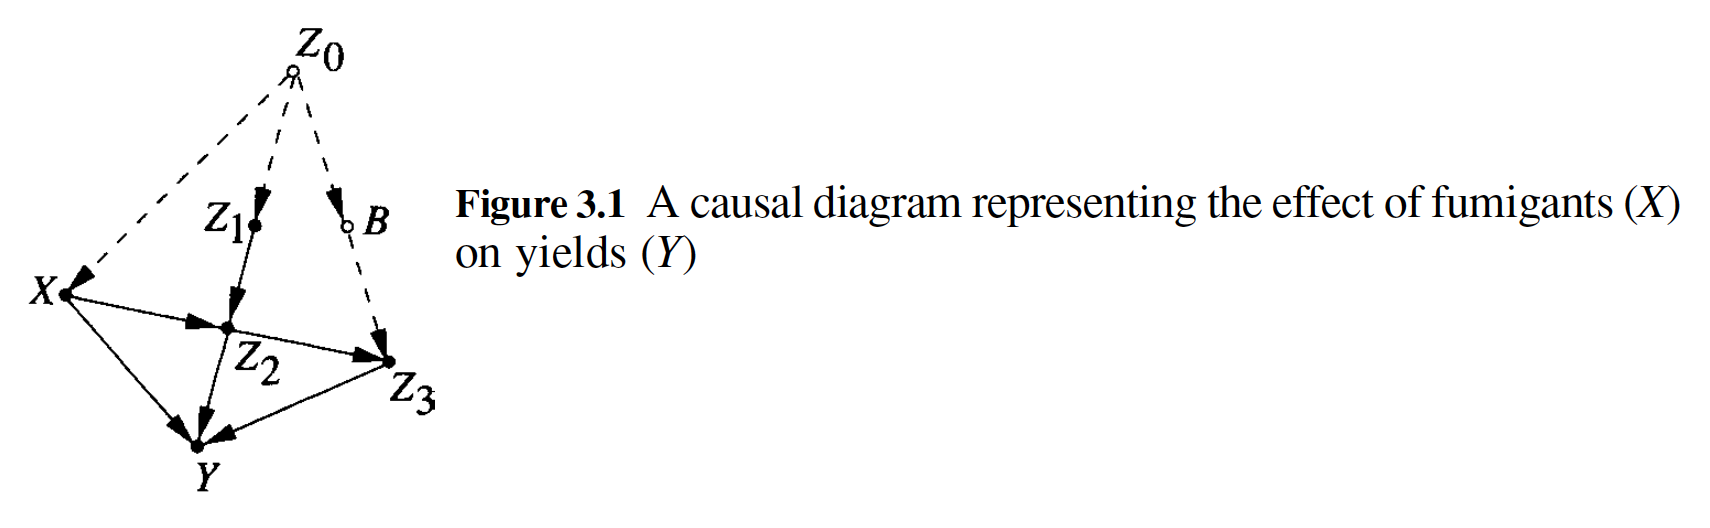
\includegraphics[scale=0.37]{img/fig_1}

\begin{itemize}
\item \textbf{Dashed Arrows:} Emanating from unmeasured quantities
\item \textbf{Solid Arrows:} Connecting measured quantities
\item \textbf{Assumptions}: The substantive assumptions embodied in the diagram are negative causal assertions which are conveyed through the links missing from the diagram
\end{itemize}
\end{frame}

\begin{frame}
The causal diagram is similar in many respects to the path diagrams devised by Wright (1921). Many similarities. The major differences lie in the method of analysis:
\begin{itemize}
\item First, whereas path diagrams have been analyzed mostly in the context of linear models with Gaussian noise, causal diagrams permit arbitrary nonlinear interactions
\item Second, causal diagrams will be used not only as a passive language to communicate assumptions but also as an active computational device through which the desired quantities are derived where $P(y \mid \hat{x})$ stands for the probability of achieving a yield level of $Y=y$, given that the treatment is set to level $X=x$ by external intervention
\end{itemize}

\begin{center}
[Demonstration On the Board]
\end{center}

These conclusions will be obtained either by analyzing the graphical properties of the diagram or by performing a sequence of symbolic derivations (governed by the diagram) that gives rise to causal effect formulas.
\end{frame}


\begin{frame}
\frametitle{2. Intervention in Markovian Models}
\begin{itemize}
\item In Chapter 1, we saw how causal models, unlike probabilistic models, can serve to predict the effect of interventions
\item This added feature requires that the joint distribution $P$ be supplemented with a causal diagram - that is, a directed acyclic graph $G$ that identifies the causal connections among the variables of interest
\item In this section we elaborate on the nature of interventions and give explicit formulas for their effects
\end{itemize}
\end{frame}

\begin{frame}
\frametitle{2.1 Graphs as Models of Interventions}
The connection between the causal and associational readings of DAGs is formed through the mechanism-based account of causation. Pearl and Verma (1991) interpreted the causal reading of a DAG in terms of functional, rather than probabilistic (see Chapter 2).
\begin{itemize}
\item In other words, each child-parent family in a DAG $G$ represents a deterministic function
$$
x_i=f_i\left(p a_i, \varepsilon_i\right), \quad i=1, \ldots, n,
$$
where $pa_i$ are the parents of variable $X_i$ in $G$.
\item The $\varepsilon_i(1 \leq i \leq n)$ are jointly independent, arbitrarily distributed random disturbances. These disturbance terms represent independent background factors that the investigator chooses not to include in the analysis.
\end{itemize}

\begin{center}
[Demonstration On the Board]
\end{center}
\end{frame}

\begin{frame}
A full specification of a causal model would entail two components
\begin{itemize}
\item A set of functional relationships
$$
x_i=f_i\left(p a_i, u_i\right), \quad i=1, \ldots, n,
$$
\item A joint distribution function $P(u)$ on the background factors
\end{itemize}

The functional characterization of each childparent relationship leads to the same recursive decomposition of the joint distribution that characterizes Bayesian networks.
\begin{center}
[Demonstration On the Board]
\end{center}

\vspace{0.2cm}
\begin{itemize}
\item If the diagram $G(M)$ associated with a causal model $M$ is acyclic, then $M$ is called \textbf{semi-Markovian}.
\item If, in addition, the background variables are independent, $M$ is called \textbf{Markovian}, since the resulting distribution of the observed variables would then be Markov relative to $G(M)$ (see Theorem 1.4.1).
\end{itemize}
\end{frame}

\begin{frame}
\textbf{Interventions}
\vspace{0.2cm}
\begin{itemize}
\item The simplest type of external intervention is one in which a single variable, say $X_i$, is forced to take on some fixed value $x_i$ (which we call "atomic")
\item Formally, this atomic intervention, which we denote by $do\left(X_i=x_i\right)$, or $do\left(x_i\right)$ for short, amounts to removing the equation $x_i=f_i\left(p a_i, u_i\right)$ from the model and substituting $X_i=x_i$ in the remaining equations
\item When solved for the distribution of $X_j$, yields the causal effect of $X_i$ on $X_j$, which is denoted $P\left(x_j \mid \hat{x}_i\right)$
\end{itemize}

This argument can be generalized to a subset $X$ of variables to attain fixed values $x$, then a subset of equations is to be pruned from the model...
\end{frame}

\begin{frame}
\textbf{Causal Effect}

\vspace{0.2cm}
Now we can formally define the causal effect...
\vspace{0.2cm}

\textbf{Definition (Causal Effect):} Given two disjoint sets of variables, $X$ and $Y$, the causal effect of $X$ on $Y$, denoted either as $P(y \mid \hat{x})$ or as $P(y \mid d o(x))$, is a function from $X$ to the space of probability distributions on $Y$. For each realization $x$ of $X, P(y \mid \hat{x})$ gives the probability of $Y=y$ induced by deleting from the model of $x_i=f_i\left(p a_i, u_i\right)$ all equations corresponding to variables in $X$ and substituting $X=x$ in the remaining equations.
\end{frame}

\begin{frame}
\frametitle{2.2 Interventions as Variables (Side Track)}
An alternative (but sometimes more appealing) account of intervention treats the force responsible for the intervention as a variable within the system (Pearl 1993b). This is facilitated by representing the function $f_i$ itself as a value of a variable $F_i$, hence
$$
x_i=I\left(p a_i, f_i, u_i\right),
$$
where $I$ is a three-argument function satisfying $I(a, b, c)=f_i(a, c)$ whenever $b=f_i$.
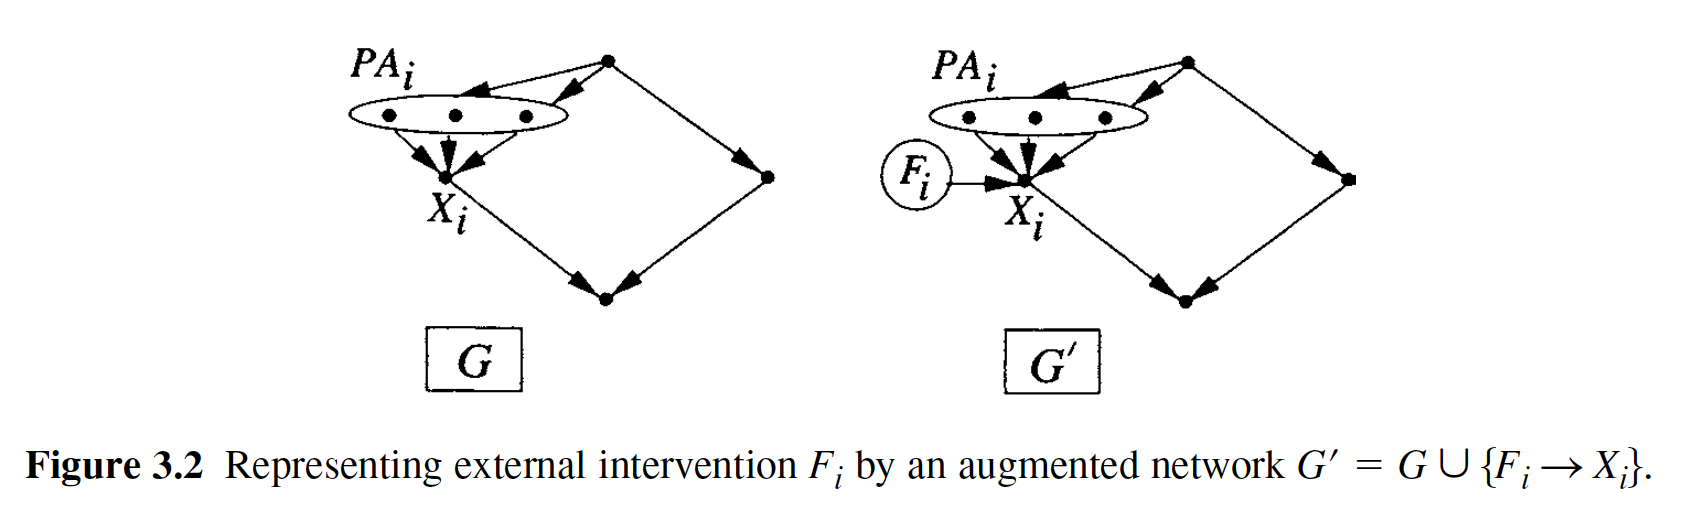
\includegraphics[scale=0.37]{img/fig_2}
\end{frame}

\begin{frame}
\begin{itemize}
\item Graphically, we can represent $F_i$ as an added parent node of $X_i$, and the effect of such an intervention can be analyzed by standard conditionalization
\item This amounts to conceptualizing the intervention as an external force $F_i$ that alters the function $f_i$ between $X_i$ and its parents
\item The advantage of the augmented network representation is that it is applicable to any change in the functional relationship $f_i$ and not merely to the replacement of $f_i$ by a constant
\end{itemize}
\end{frame}

\begin{frame}
\frametitle{2.3 Computing the Effect of Interventions}
Regardless of whether we represent interventions as a modification of an existing model or as a conditionalization in an augmented model, the result is a well-defined transformation between the preintervention and postintervention distributions.

\vspace{0.3cm}
\textbf{Atomic Intervention:} In the case of an atomic intervention $do\left(X_i=x_i^{\prime}\right)$, this transformation can be expressed in a simple truncated factorization formula
$$
P\left(x_1, \ldots, x_n \mid \hat{x}_i^{\prime}\right)= \begin{cases}\prod_{j \neq i} P\left(x_j \mid p a_j\right) & \text { if } x_i=x_i^{\prime}, \\ 0 & \text { if } x_i \neq x_i^{\prime}\end{cases}
$$

\begin{itemize}
\item The equation reflects the removal of the term $P\left(x_i \mid p a_i\right)$ from the product, since $p a_i$ no longer influences $X_i$
\item Graphically, the removal of the term $P\left(x_i \mid p a_i\right)$ is equivalent to removing the links between $P A_i$ and $X_i$ while keeping the rest of the network intact
\end{itemize}
\end{frame}

\begin{frame}
Multiplying and dividing the equation by $P\left(x_i^{\prime} \mid p a_i\right)$, the relationship to the preintervention distribution becomes more transparent:
$$
P\left(x_1, \ldots, x_n \mid \hat{x}_i^{\prime}\right)= \begin{cases}\frac{P\left(x_1, \ldots, x_n\right)}{P\left(x_i^{\prime} \mid p a_i\right)} & \text { if } x_i=x_i^{\prime}, \\ 0 & \text { if } x_i \neq x_i^{\prime}\end{cases}
$$

Each point $\left(x_1, \ldots, x_n\right)$ is seen to increase its mass by a factor equal to the inverse of the conditional probability $P\left(x_i^{\prime} \mid p a_i\right)$ corresponding to that point (mass transfered from excluded point $\left(x_i \neq x_i^{\prime} \right)$ to a select set of points that share the same value of $p a_i$)

\begin{itemize}
\item Points for which this conditional probability is low would boost their mass value substantially
\item Points possessing a $p a_i$ value that anticipates a natural (noninterventional) realization of $x_i^{\prime}$
\end{itemize}
\end{frame}

\begin{frame}
Another interesting form obtains when we interpret the division by $P\left(x_i^{\prime} \mid\right.$ $\left.p a_i\right)$ as conditionalization on $x_i^{\prime}$ and $p a_i$:
$$
P\left(x_1, \ldots, x_n \mid \hat{x}_i^{\prime}\right)= \begin{cases}P\left(x_1, \ldots, x_n \mid x_i^{\prime}, p a_i\right) P\left(p a_i\right) & \text { if } x_i=x_i^{\prime}, \\ 0 & \text { if } x_i \neq x_i^{\prime}\end{cases}
$$

Summing over all variables except $Y \cup X_i$ yields the following:
\vspace{0.2cm}

\textbf{Theorem (Adjustment for Direct Causes):} Let $P A_i$ denote the set of direct causes of variable $X_i$ and let $Y$ be any set of variables disjoint of $\left\{X_i \cup P A_i\right\}$. The effect of the intervention do $\left(X_i=x_i^{\prime}\right)$ on $Y$ is given by
$$
P\left(y \mid \hat{x}_i^{\prime}\right)=\sum_{p a_i} P\left(y \mid x_i^{\prime}, p a_i\right) P\left(p a_i\right),
$$
where $P\left(y \mid x_i^{\prime}, p a_i\right)$ and $P\left(p a_i\right)$ represent preintervention probabilities.
\end{frame}

\begin{frame}
\frametitle{2.4 Identification of Causal Quantities}
Causal quantities, unlike statistical parameters, are defined relative to a \textbf{causal model} $M$ and not relative to a \textbf{joint distribution} $P_M(\dot{v})$ over the set $V$ of observed variables. The desired quantity will not be discernible unambiguously from the data - even when infinitely many samples are taken.

\vspace{0.4cm}
\textbf{Identifiability} ensures that the added assumptions conveyed by $M$ will supply the missing information without explicating $M$ in full.
\end{frame}

\begin{frame}
\textbf{Definition: (Identifiability)} Let $Q(M)$ be any computable quantity of a model $M$. We say that $Q$ is identifiable in a class $\boldsymbol{M}$ of models if, for any pairs of models $M_1$ and $M_2$ from $\boldsymbol{M}, Q\left(M_1\right)=Q\left(M_2\right)$ whenever $P_{M_1}(v)=P_{M_2}(v)$. If our observations are limited and permit only a partial set $F_M$ of features (of $P_M(v)$) to be estimated, we define $Q$ to be identifiable from $F_M$ if $Q\left(M_1\right)=Q\left(M_2\right)$ whenever $F_{M 1}=F_{M 2}$.

\vspace{0.4cm}
Identifiability is essential for integrating statistical data (summarized by $P(v)$) with incomplete causal knowledge of $\left\{f_i\right\}$, as it enables us to estimate quantities $Q$ consistently from large samples of $P(v)$ without specifying the details of $M$.

\vspace{0.4cm}
For the purpose of our analysis, the quantity $Q$ of interest is the causal effect $P_M(y \mid \hat{x})$.
\end{frame}

\begin{frame}
\textbf{Definition (Causal Effect Identifiability):} The causal effect of $X$ on $Y$ is identifiable from a graph $G$ if the quantity $P(y \mid \hat{x})$ can be computed uniquely from any positive probability of the observed variables - that is, if $P_{M_1}(y \mid \hat{x})=P_{M_2}(y \mid \hat{x})$ for every pair of models $M_1$ and $M_2$ with $P_{M_1}(v)=P_{M_2}(v)>$ 0 and $G\left(M_1\right)=G\left(M_2\right)=G$.

\vspace{0.4cm}
The identifiability of $P(y \mid \hat{x})$ ensures that it is possible to infer the effect of action $d o(X$ $=x)$ on $Y$ from two sources of information:
\begin{itemize}
\item Passive observations, as summarized by the probability function $P(v)$
\item The causal graph $G$, which specifies (qualitatively) which variables make up the stable mechanisms in the domain
\end{itemize}
\end{frame}

\begin{frame}
\textbf{Theorem:} Given a causal diagram $G$ of any Markovian model in which a subset $V$ of variables are measured, the causal effect $P(y \mid \hat{x})$ is identifiable whenever $\left\{X \cup Y \cup P A_X\right\} \subseteq V$, that is, whenever $X, Y$, and all parents of variables in $X$ are measured. The expression for $P(y \mid \hat{x})$ is then obtained by adjusting for $P A_x$.

\vspace{0.4cm}
\textbf{Corollary:} Given the causal diagram $G$ of any Markovian model in which all variables are measured, the causal effect $P(y \mid \hat{x})$ is identifiable for every two subsets of variables $X$ and $Y$.

\vspace{0.4cm}
We now turn our attention to identification problems in semi-Markovian models.
\end{frame}

\begin{frame}
\frametitle{3. Controlling Confounding Bias}
\begin{itemize}
\item Whenever we undertake to evaluate the effect of one factor $(X)$ on another $(Y)$, the question arises as to whether we should adjust our measurements for possible variations in some other factors $(Z)$ (known as confounders)
\item Adjustment amounts to partitioning the population into groups that are homogeneous relative to $Z$, assessing the effect of $X$ on $Y$ in each homogeneous group, and then averaging the results
\item \textbf{Simpson's paradox:} Any statistical relationship between two variables may be reversed by including additional factors in the analysis.
\end{itemize}
\end{frame}

\begin{frame}
Pearl's criticism of the potential-outcome framework...

\vspace{0.4cm}
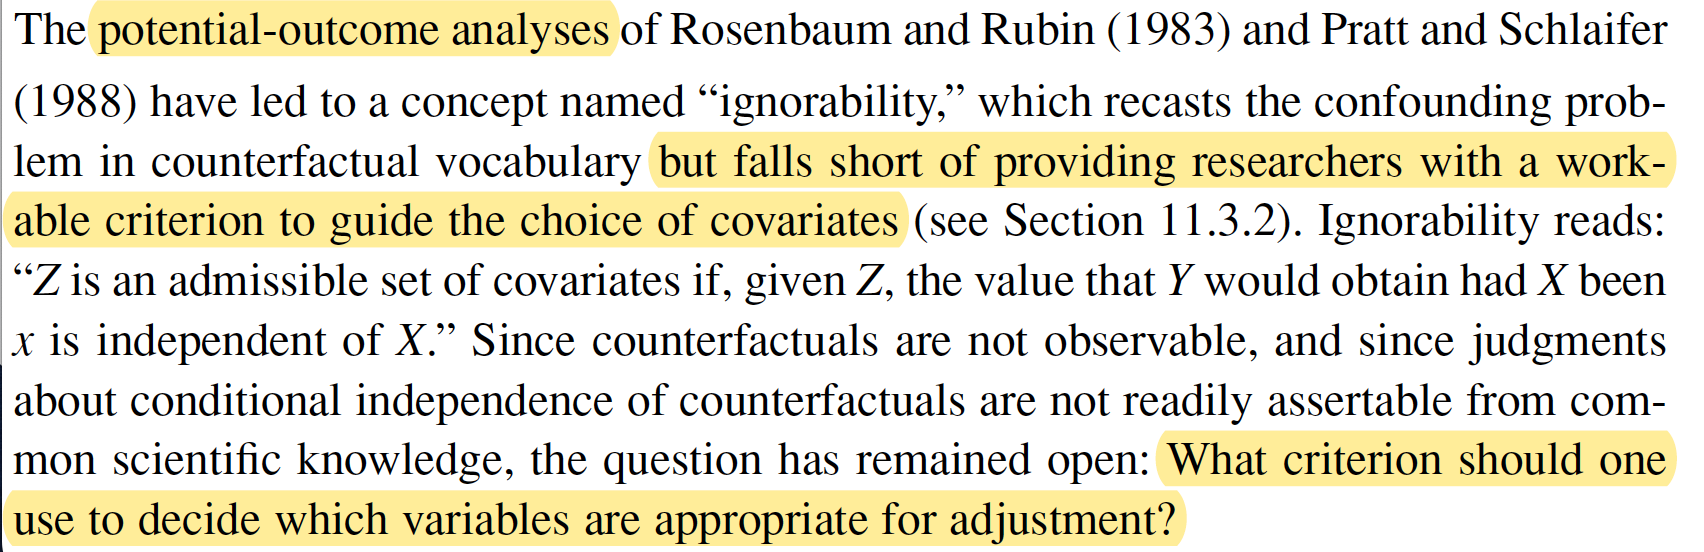
\includegraphics[scale=0.37]{img/fig_3}

\vspace{0.4cm}
[Reference: Page 79]
\end{frame}

\begin{frame}
\frametitle{3.1 The Back-Door Criterion}
\vspace{0.3cm}
\textbf{Definition: (Back-Door)} A set of variables $Z$ satisfies the back-door criterion relative to an ordered pair of variables $\left(X_i, X_j\right)$ in a DAG $G$ if:
\begin{itemize}
\item no node in $\mathrm{Z}$ is a descendant of $X_i$
\item $Z$ blocks every path between $X_i$ and $X_j$ that contains an arrow into $X_i$.
\end{itemize}

\vspace{0.4cm}
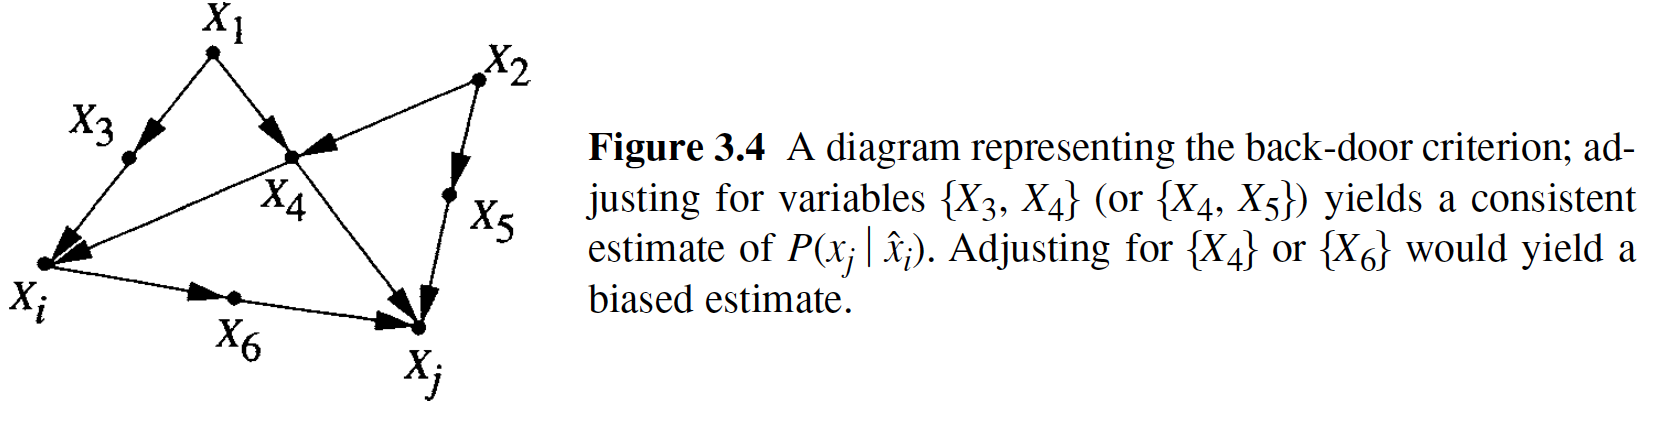
\includegraphics[scale=0.37]{img/fig_4}
\end{frame}

\begin{frame}
\vspace{0.3cm}
\textbf{Theorem: (Back-Door Adjustment)} If a set of variables $Z$ satisfies the back-door criterion relative to $(X, Y)$, then the causal effect of $X$ on $Y$ is identifiable and is given by the formula
$$
P(y \mid \hat{x})=\sum_z P(y \mid x, z) P(z)
$$
\end{frame}


\begin{frame}
\frametitle{3.2 The Front-Door Criterion}
\textbf{Definition (Front-Door):} A set of variables $Z$ is said to satisfy the front-door criterion relative to an ordered pair of variables $(X, Y)$ if:
\begin{itemize}
\item $Z$ intercepts all directed paths from $X$ to $Y$
\item there is no unblocked back-door path from $X$ to $\mathrm{Z}$
\item all back-door paths from $Z$ to $Y$ are blocked by $X$
\end{itemize}

\vspace{0.4cm}
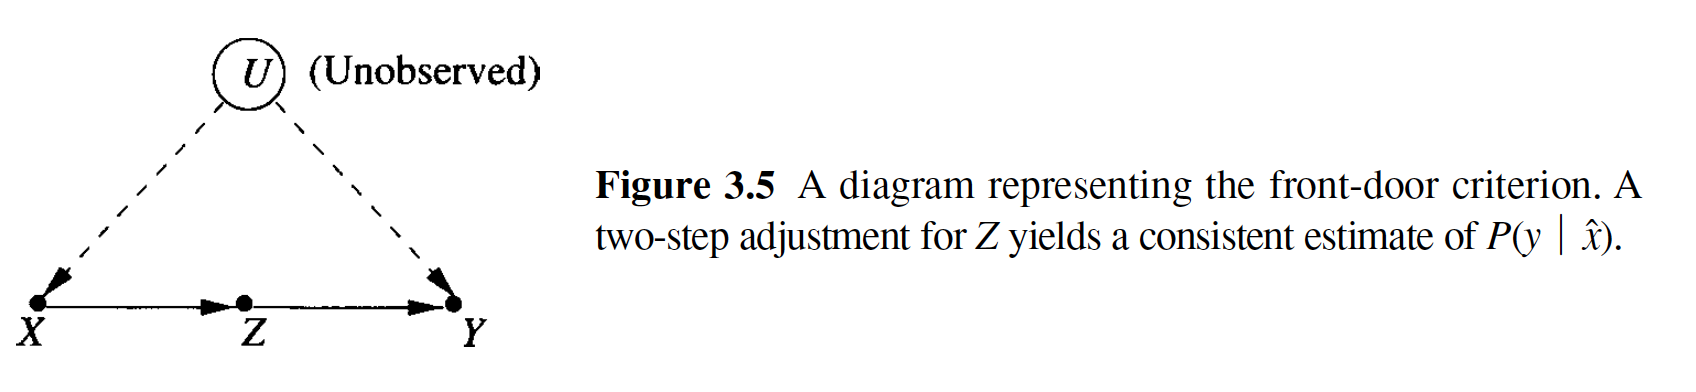
\includegraphics[scale=0.37]{img/fig_5}
\end{frame}

\begin{frame}
\vspace{0.3cm}
\textbf{Theorem (Front-Door Adjustment):} If $Z$ satisfies the front-door criterion relative to $(X, Y)$ and if $P(x, z)>0$, then the causal effect of $X$ on $Y$ is identifiable and is given by the formula
$$
P(y \mid \hat{x})=\sum_z P(z \mid x) \sum_{x^{\prime}} P\left(y \mid x^{\prime}, z\right) P\left(x^{\prime}\right)
$$

\textbf{Comment:} The front-door adjustment can be interpreted as a two-step application of the back-door formula.
\end{frame}

\begin{frame}
\frametitle{Example: Smoking and the Genotype Theory}
Consider the century-old debate on the relation between smoking (X) and lung cancer (Y). According to many, the tobacco industry has managed to forestall antismoking legislation by arguing that the observed correlation between smoking and lung cancer could be explained by some sort of carcinogenic genotype $(U)$ that involves inborn craving for nicotine
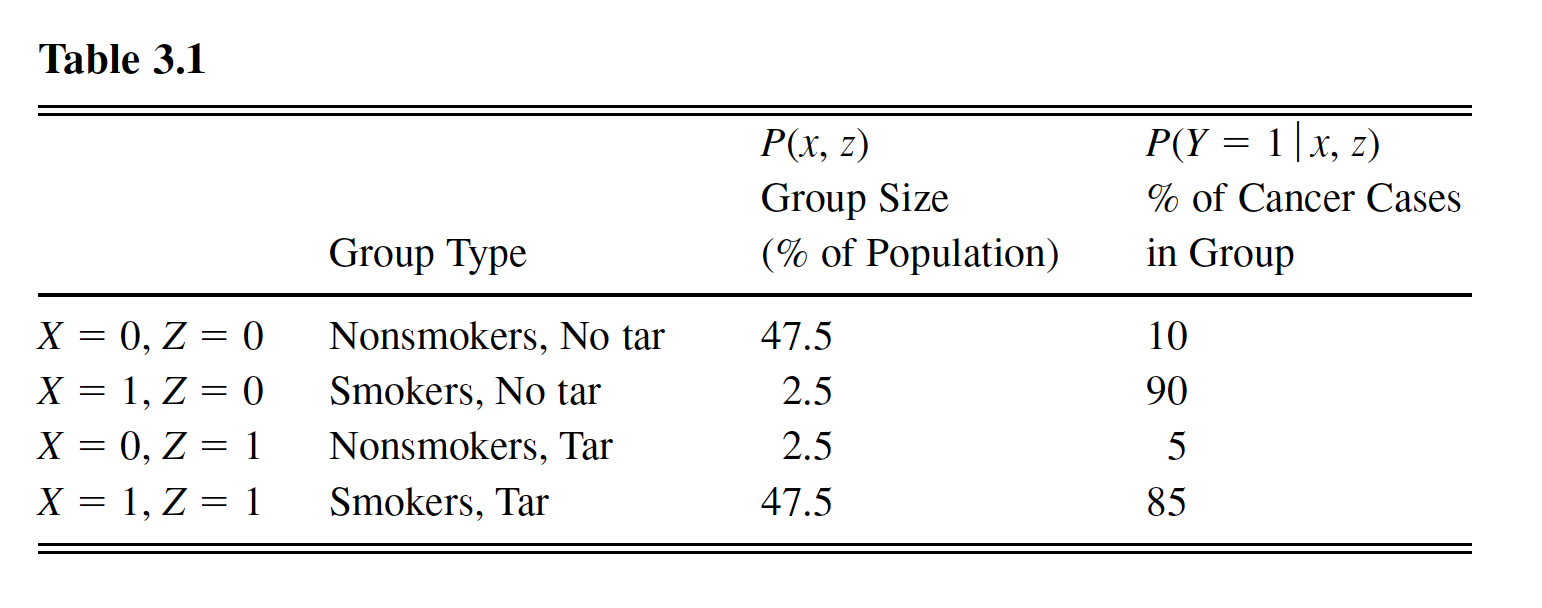
\includegraphics[scale=0.37]{img/fig_6}
\end{frame}

\begin{frame}
The amount of $\operatorname{tar}(Z)$ deposited in a person's lungs is a variable that promises to meet the conditions listed in front-door criterion.
\begin{itemize}
\item Smoking cigarettes has no effect on the production of lung cancer except as mediated through tar deposits
\item Even if a genotype is aggravating the production of lung cancer, it nevertheless has no effect on the amount of tar in the lungs except indirectly (through cigarette smoking)
\item Likewise, we must assume that no other factor that affects tar deposit has any influence on smoking
\item Finally, condition $P(x, z)>0$ requires that high levels of tar in the lungs be the result not only of cigarette smoking but also of other factors (e.g., exposure to environmental pollutants)
\end{itemize}
\end{frame}

\begin{frame}
Substituting the appropriate values of $P(z \mid x), P(y \mid x, z)$, and $P(x)$, we have
$$
P(Y=1 \mid d o(X=1))=.4525
$$
$$
P(Y=1 \mid d o(X=0))=.4975
$$
\begin{itemize}
\item The table shows that tar deposits have a protective effect in both groups: in smokers, tar deposits lower cancer rates from $90 \%$ to $85 \%$, in nonsmokers, they lower cancer rates from $10 \%$ to $5 \%$
\item Thus, regardless of whether I have a natural craving for nicotine, I should be seeking the protective effect of tar deposits in my lungs, and smoking offers a very effective means of acquiring those deposits
\end{itemize}

\vspace{0.3cm}
\textbf{Conclusion:} Thus, contrary to expectation, the data prove smoking to be somewhat beneficial to one's health.
\end{frame}

\begin{frame}
\textbf{What's Wrong?}

\vspace{0.3cm}
The purpose of this exercise was to demonstrate how reasonable qualitative assumptions about the workings of mechanisms, coupled with nonexperimental data, can produce precise quantitative assessments of causal effects.

\begin{itemize}
\item In reality, we would expect observational studies involving mediating variables to refute the genotype theory by showing, for example, that the mediating consequences of smoking (such as tar deposits) tend to increase, not decrease, the risk of cancer in smokers and nonsmokers alike.
\end{itemize}
\end{frame}

\begin{frame}
\frametitle{4. A Calculus of Intervention}
This section establishes a set of inference rules by which probabilistic sentences involving interventions and observations can be transformed into other such sentences, thus providing a syntactic method of deriving (or verifying) claims about interventions.
\begin{itemize}
\item We will assume that we are given the structure of a causal diagram $G$ in which some of the nodes are observable while others remain unobserved
\item Our objective will be to facilitate the syntactic derivation of causal effect expressions of the form $P(y \mid \hat{x})$, where $X$ and $Y$ stand for any subsets of observed variables
\item By "derivation" we mean stepwise reduction of the expression $P(y \mid \hat{x})$ to an equivalent expression involving standard probabilities of observed quantities
\end{itemize}
Whenever such reduction is feasible, the causal effect of $X$ on $Y$ is identifiable.
\end{frame}

\begin{frame}
\frametitle{4.1 Preliminary Notation}
Let $X, Y$, and $Z$ be arbitrary disjoint sets of nodes in a causal DAG $G$.
\begin{itemize}
\item We denote by $G_{\bar{X}}$ the graph obtained by deleting from $G$ all arrows pointing to nodes in $X$
\item Likewise, we denote by $G_{\underline{X}}$ the graph obtained by deleting from $G$ all arrows emerging from nodes in $X$
\item To represent the deletion of both incoming and outgoing arrows, we use the notation $G_{\bar{X} \underline{Z}}$
\end{itemize}
Finally, the expression $P(y \mid \hat{x}, z) \triangleq$ $P(y, z \mid \hat{x}) / P(z \mid \hat{x})$ stands for the probability of $Y=y$ given that $X$ is held constant at $x$ and that (under this condition) $Z=z$ is observed.
\end{frame}

\begin{frame}
\frametitle{4.2 Inference Rules}
\textbf{Theorem (Rules of do Calculus):} Let $G$ be the directed acyclic graph associated with a causal model as defined in, and let $P(\cdot)$ stand for the probability distribution induced by that model. For any disjoint subsets of variables $X, Y, Z$, and $W$, we have the following rules.
\begin{itemize}
\item \textbf{Rule 1 (Insertion/deletion of observations):}
$$
P(y \mid \hat{x}, z, w)=P(y \mid \hat{x}, w) \quad \text { if }(Y \perp Z) \mid X, W)_{G_{\bar{X}}}
$$
\item \textbf{Rule 2 (Action/observation exchange):}
$$
P(y \mid \hat{x}, \hat{z}, w)=P(y \mid \hat{x}, z, w) \quad if (Y \perp Z) \mid X, W)_{G_{\bar{X}} \underline{z}}
$$
\item \textbf{Rule 3 (Insertion/deletion of actions):}
$$
P(y \mid \hat{x}, \hat{z}, w)=P(y \mid \hat{x}, w) \text { if }(Y \perp Z \mid X, W)_{G_{\bar{X}, \overline{Z(W)}}}
$$
where $Z(W)$ is the set of $Z$-nodes that are not ancestors of any $W$-node in $G_{\bar{X}}$.
\end{itemize}
\end{frame}

\begin{frame}
\frametitle{Example: Symbolic Derivation of Causal Effects}
We will now demonstrate how Rules 1-3 can be used to derive all causal effect estimands in the structure
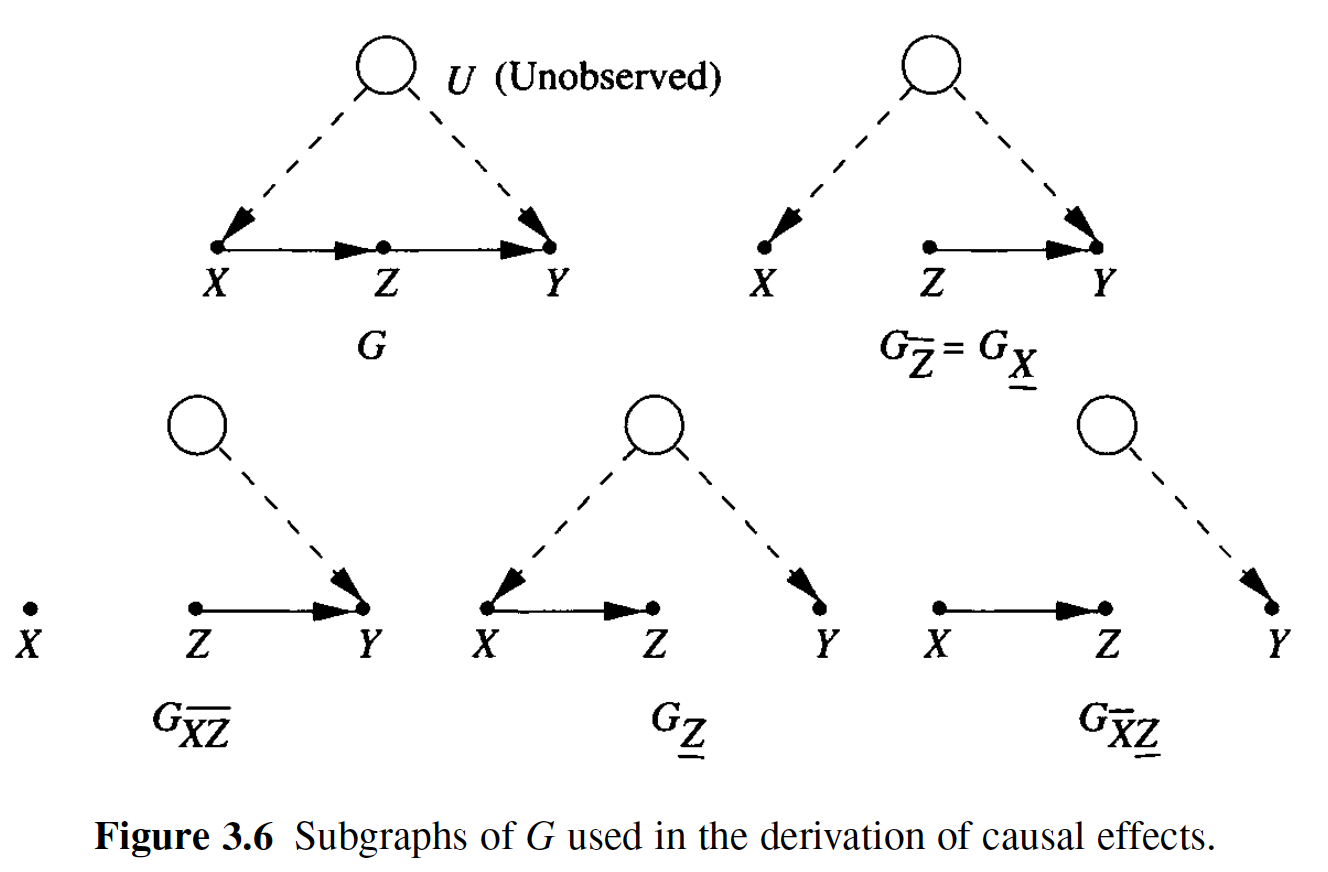
\includegraphics[scale=0.45]{img/fig_7}
\begin{center}
[Demonstration On the Board]
\end{center}
\end{frame}
\end{document}
